\documentclass{article}
\usepackage[utf8]{inputenc}
\usepackage{mathtools}
\usepackage{amsmath}
\usepackage{amssymb}
\usepackage{witharrows}
\usepackage{cancel}
\usepackage{systeme}
\usepackage{mathrsfs}
\usepackage{subcaption}
\newcommand{\norm}[1]{\left\lVert#1\right\rVert}
\newcommand{\eunorm}[1]{\left\lVert#1\right\rVert_{2}}
\newcommand{\anglepar}[1]{\left\langle#1\right\rangle}
\newcommand{\absolute}[1]{\left\lvert#1\right\rvert}
\newtheorem{definition}{Definition}
\newtheorem{remark}{Remark}
\newtheorem{theorem}{Theorem}
\newtheorem{proof}{Proof}
\newtheorem{lemma}{Lemma}
\newtheorem{corollary}{Corollary}

\title{Fundamentals of Neural Networks}
\author{Pietro Marcatti}
\date{First Semester 2022/2023}
\makeindex

\begin{document}
\maketitle
\section*{Introduction}
\section*{Linear Algebra - A Mathematical Background}
A mind-map summarising the key concept of this chapter and their relationship:
\begin{figure}[htbp]
    \centering
    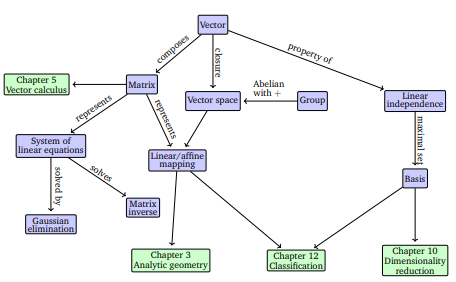
\includegraphics[width= 12cm]{Mathematical Background/mind-map.png}
\end{figure}

\subsection*{Systems of Linear Equations}
Systems of linear equations play a central part of linear algebra. Many problems can be formulated as systems of linear equations, and linear algebra gives us the tools for solving them.\\
In general, for a real-valued system of linear equations we obtain either no, exactly one, or infinitely many solutions. We can introduce a useful compact notation for systems of linear equations ($SLE$) collecting the coefficients $a_{ij}$ into vectors and collect the vectors into matrices.
\begin{align}
    \begin{bmatrix}
        a_{11}\\
        \vdots\\
        a_{m1}
    \end{bmatrix} x_1
    + \begin{bmatrix}
        a_{12}\\
        \vdots\\
        a_{m2}
    \end{bmatrix} x_2
    +\cdots&+
    \begin{bmatrix}
        a_{1n}\\
        \vdots\\
        a_{mn}
    \end{bmatrix} x_n
    = \begin{bmatrix}
        b_{1}\\
        \vdots\\
        b_{m}
    \end{bmatrix}
\end{align}
\begin{align}
    \Longleftrightarrow
    \begin{bmatrix}
        a_{11}& \cdots & a_{1n}\\
        \vdots& & \vdots\\
        a_{m1}& \cdots & a_{mn}
    \end{bmatrix}
    \begin{bmatrix}
        x_{1}\\
        \vdots\\
        x_{m}
    \end{bmatrix}
    &= \begin{bmatrix}
        b_{1}\\
        \vdots\\
        b_{m}
    \end{bmatrix}
\end{align}
\begin{definition}[Homogeneous SLE]
    A system of linear equations is defined as homogeneous if $\vec{b} = \vec{0}$
\end{definition}
%%%%%%%%%%%%%%%%%%%%%%%%%%%%%%%%%%%%%%%%%%
\subsection*{Matrices}
Matrices play a central role in linear algebra and other than to compactly represent $SLE$s they can be used to represent linear functions (linear mappings).

\begin{definition}[Matrix]
    With $m,n \in \mathbb{N}$ a real-valued $(m,n)$ matrix \textbf{A} is an $m\cdot n$-tuple of elements $a_{ij}, i=1,\ldots,n, j=1,\ldots,n$ which is ordere according to a rectangular scheme consisting of $m$ rows and $n$ columns:
\end{definition}
\begin{align}
    \mathbf{A} =
    \begin{bmatrix}
        a_{11} & a_{12} & \cdots & a_{1n}\\
        a_{21} & a_{22} & \cdots & a_{2n}\\
        \vdots & \vdots &  & \vdots\\
        a_{m1} & a_{m2} & \cdots & a_{mn}
    \end{bmatrix}, \quad a_{ij} \in \mathbb{R}
\end{align}
By convention $(1,n)$-matrices are called rows and $(m,1)$-matrices are called columns. These special matrices are also called row/column vectors.\\
For matrices $\mathbf{A} \in \mathbb{R}^{m\times n},\mathbf{B} \in \mathbb{R}^{n\times k}$, the elements $c_{ij}$ of the product $\mathbf{C} = \mathbf{AB} \in \mathbb{R}^{m\times k}$ are computed as follows:
\[
    c_{ij}= \sum_{l=1}^{n}{a_{il}b_{lj}}, \quad i=1,\ldots,m \quad j=1, \ldots, k  
\]
This means that the elements of the $i$th-row of \textbf{A} are multiplied with the elements of the $j$th-column of \textbf{B} and then summed together.
\begin{definition}[Identity Matrix]
    In $\mathbb{R}^{n\times n}$, we define the identity matrix as the $n \times n$ matrix containing 1 on the diagonal and 0 everywhere else. 
\end{definition}
With the understanding of matrix multiplication, matrix addition and the identity matrix we can take a look at some properties of matrices:
\begin{description}
    \item[Associativiy:]\[
        \forall \mathbf{A} \in \mathbb{R}^{m\times n}, \mathbf{B} \in \mathbb{R}^{n\times p}, \mathbf{C} \in \mathbb{R}^{p\times q}: (\mathbf{AB})\mathbf{C} = \mathbf{A}(\mathbf{BC})
    \]
    \item[Distributivity] \begin{align}
        \forall \mathbf{A,B} \in \mathbb{R}^{m\times n}, \mathbf{C,D} \in \mathbb{R}^{n\times p}: &(\mathbf{A}+\mathbf{B})\mathbf{C}= \mathbf{AC}+\mathbf{BC} \\ 
        &\mathbf{A}(\mathbf{C}+\mathbf{D})= \mathbf{AC}+\mathbf{AD}
    \end{align}
\end{description}
\begin{definition}[Inverse]
    Consider a square matrix $\mathbf{A} \in \mathbb{R}^{n\times n}$. Let matrix $\mathbf{B} \in \mathbb{R}^{n\times n}$ have the property that $\mathbf{AB} = \mathbf{I}_n = \mathbf{BA}$. $\mathbf{B}$ is called the inverse of $\mathbf{A}$ and denoted by $\mathbf{A}^{-1}$
\end{definition}
Unfortunately not every matrix possesses and inverse. If this inverse does exist the matrix is called regular/invertible/nonsingular; otherwise it's called singular/noninvertible.
\begin{definition}[Transpose]
    For $\mathbf{A} \in \mathbb{R}^{m\times n}$ the matrix $\mathbf{B} \in \mathbb{R}^{n\times m}$ with $b_{ij}= a_{ji}$ is called the transpose of $\mathbf{A}$. We write it as $\mathbf{B} = \mathbf{A}^T$
\end{definition}
\begin{definition}[Symmetric Matrix]
    A matrix $\mathbf{A} \in \mathbb{R}^{n\times n}$ is symmetric if $\mathbf{A} = \mathbf{A}^T$
\end{definition}
\subsubsection*{Compact Representations of SLE}
If we consider a system of linear equations and use the rules for matrix multiplication, we can write this equation system in a more compact form:
\[
    \begin{bmatrix}
        2 & 3 & 5 \\
        4 & -2 & -7 \\
        9 & 5 & -3
    \end{bmatrix}
    \begin{bmatrix}
        x_1 \\
        x_2\\
        x_3
    \end{bmatrix}
    =
    \begin{bmatrix}
        1 \\
        8\\
        2
    \end{bmatrix}
\]
Generally a system of linear equations can be compactly represented in their matrix form as $\mathbf{A}x=b$.\\
\begin{definition}[Row-Echelon Form REF]
    A matrix is in row-echelon form if:
    \begin{itemize}
        \item All rows that contain only zeros are at the bottom of the matrix; correspondigly, all rows that contain at least one nonzero element are on top of rows that contain only zeros.
        \item Looking at nonzero rows only, the first nonzero number from the left (also called the pivot or the leading coefficient) is always strictly to the right of the pivot of the row above it
    \end{itemize}
\end{definition}
\begin{remark}[Reduced Row-Echelon Form] An equation system is in reduced row-echelon form (also row-reduces echelon form or row canonical form) if:
    \begin{itemize}
        \item It is in row-echelon form
        \item Every pivot is 1
        \item The pivot is the only nonzero entry in its column
    \end{itemize}
\end{remark}

\subsection*{Vector Spaces}
So far we have seen that systems of linear equations can be compactly represented using matrix-vector notation. In the following chapter we will have a closer look at vector spaces, i.e., a structured space in which vectors live.
\subsubsection*{Groups}
We are ready to formalize the characteristics of vectors and scalar multiplication but we need to introduce the concept of a group. A group is a set of elements and an operation defined on these elements that keeps some structure of the set intact.
Groups play an important role in computer science. Besides providing a fundamental framework for operations on sets, they are heavily used in cryptography, coding theory and graphics.
\begin{definition}[Group]
    Consider a set $\mathcal{G}$ and an operation $\otimes: \mathcal{G} \times \mathcal{G} \rightarrow \mathcal{G}$ defined on $\mathcal{G}$. Then $G:=(\mathcal{G},\otimes)$ is called a group if the following hold:
    \begin{enumerate}
        \item Closure of $\mathcal{G}$ under $\otimes: \forall x,y \in \mathcal{G}: x\otimes y \in \mathcal{G}$
        \item Associativiy: $\forall x,y,z \in \mathcal{G}: (x\otimes y) \otimes z = x \otimes(y \otimes z)$
        \item Neutral element: $\exists e \in \mathcal{ G} \forall x \in \mathcal{G} : x\otimes e = x$ and $e \otimes x =x$
        \item Inverse element: $\forall x \in \mathcal{G} \exists y\in \mathcal{G}: x\otimes y = e$ and $y\otimes x = e$, where $e$ is the neutral element. We oftern write $x^{-1}$ to denote the inverse element of x.
    \end{enumerate}
\end{definition}
\begin{remark}[Abelian Group]
    If additionally $\forall x,y \in \mathcal{G}: x\otimes y = y\otimes x$, then $G = (\mathcal{G,\otimes})$ is an Abelian group (commutative).
\end{remark}
\subsubsection*{Vector Spaces}
We will now consider an extension of the definition of group that in addition to an inner operation $+$ also contain an outer operation $\cdot$, the multiplication of a vector $x\in \mathcal{G}$ by a scalar $\lambda \in \mathbb{R}$.
\begin{definition}[Vector space]
    A real-valued vector space $V = (\mathcal{V}, +, \cdot)$ is a set $\mathcal{V}$ with two operations
    \begin{align*}
        + : \mathcal{V} \times \mathcal{V} \rightarrow \mathcal{V}\\
        \cdot : \mathbb{R}  \times \mathcal{V} \rightarrow \mathcal{V}
    \end{align*}
    where
    \begin{enumerate}
        \item $(\mathcal{V},+)$ is an Abelian group
        \item Distributivity
        \item Associativiy (w.r.t. the outer operation)
        \item Neutral element (w.r.t. the outer operation)
    \end{enumerate}
\end{definition}
The elements $x \in V$ are called vectors.
\begin{remark}
    A "vector multiplication" $\mathbf{ab}, a,b \in \mathbb{R}^n$ is not defined. We could use the matrix multiplication as previously defined however the dimensions of the vectors do not match. Only the following multiplication for vectors are defined: $\mathbf{ab}^T \in \mathbb{R}^{n\times n}$ (outer product), $\mathbf{a^Tb}\in \mathbb{R}$ (inner/scalar/dot product)
\end{remark}

%%%%%%%%%%%%%%%%%%%%%%%%%%%%%%%%%%%%%%%%%%%%%%%%%%%%%%%%%%%%%%%%%
\subsubsection*{Vector Subspaces}
Intuitively, vector subspaces are sets contained in the original vector space with the property that when we perform space operations on elements within this subspace, we will never leave it. In this sense they are "closed". We will see how we can use vector subspaces to perform dimensionality reduction.
\begin{definition}[Vector subspace]
    Let $V = (\mathcal{V}, +, \cdot)$ be a vector space and $\mathcal{U} \subseteq \mathcal{V}, \mathcal{U} \neq \emptyset$. Then $U = (\mathcal{U},+,\cdot)$ is called vector subspace of V (or linear subspace) if $U$ is a vector space with the vector space operations + and $\cdot$ restricted to $\mathcal{U} \times \mathcal{U}$ and $\mathbb{R} \times \mathcal{U}$. We write $U \subseteq V$ to denote a subspace $U$ of $V$.
\end{definition}
If $U$ is a vector subspace of $V$ it naturally inherits many of its properties but to determine whether $(\mathcal{U}, +, \cdot)$ is a subspace of V we still need to show
\begin{enumerate}
    \item $\mathcal{U} \neq \emptyset$, in particular $\vec{0} \in \mathcal{U}$
    \item Closure of $U$:
    \begin{enumerate}
        \item W.r.t. to the outer operation: $\forall \lambda \in \mathbb{R} \forall x \in \mathcal{U}: \lambda x \in \mathcal{U}$
        \item W.r.t. to the outer operation: $\forall x,y \in \mathcal{U}: x + y \in \mathcal{U}$
    \end{enumerate}
\end{enumerate}
Example:
\begin{figure}[htbp]
    \centering
    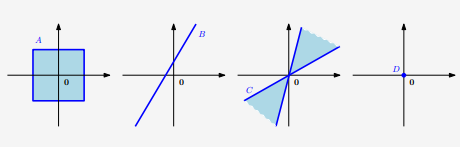
\includegraphics[width=10cm]{Mathematical Background/example-subspace-recognition.png}
\end{figure}
Only example D in the followin figureì is a subspace of $R^2$ (with the inner/outer operations). In A and C the closure property is violated, meanwhile B does not contain $\vec{0}$.
\begin{remark}
    Every subspace $U \subseteq (R^n, + ,\cdot)$ is the solution space of a homogeneous SLE $\mathbf{A}\vec{x} = \vec{0}$ for $\vec{x} \in R^n$
\end{remark}
\subsubsection*{Linear Indipendence}
In the following subsection we will take a closer look at what we can do with vectors. In particular, we can add vectors together and multiply them with scalars. The closure property guarantees that we end up with another vector in the same vector space. It is possible, we will see, to find a set of vectors with which we can represent every vector in the vector space by adding them together and scaling them. This set of vectors is a basis. Before we can explore further these concept we need to define linear combinations and linear indipendence.

\begin{definition}[Linear combination]
    Consider a vector space $V$ and a finite number of vectors $x_1,\ldots, x_k \in V$. Then, every $v \in V$ of the form
    \[
        v = \lambda_1x_1 + \cdots + \lambda_kx_k = \sum_{i=1}^{k}{\lambda_ix_i} \in V
    \] 
    with $\lambda_1,\ldots,\lambda_k \in \mathbb{R}$ is a linear combination of the vectors $x_1,\ldots, x_k$
\end{definition}
The $\vec{0}$ can always be written as the linear combination of $k$ vectors, only some of them are non-trivial. In the following we are interested in non-trivial linear combinations that represent $\vec{0}$, that is, where not all $\lambda_i$ are 0.
\begin{definition}[Linear (In)dependence]
    Let us consider a vector space $V$ with $k \in \mathbb{N}$ and $x_i, \ldots, x_k \in V$. If there is a non-trivial linear combination, such that $\vec{0} = \sum_{i=1}^{k}{\lambda_ix_i}$ with at least one $\lambda_i \neq 0$, the vectors $x_1,\ldots, x_k$ are linearly dependent. If only the trivial solution exists the vectors $x_1, \ldots, x_k$ are linearly independent.
\end{definition}
Intuitively a set of linearly independent vectors consists of vectors that have no redundancy. If we remove any of those vectors from the set, we will lose something.
\begin{remark}
    Consider a vector space $V$ with $k$ linearly independent vectors $b_1,\ldots,b_k$ and $m$ linear combinations
    \[
        x_j = \sum_{i=1}^{k}{\lambda_i1b_i}, \quad j= 1,\ldots, m
    \]
    Defining $\mathbf{B} = [b_1,\ldots,b_k]$ as the matrix whose columns are the linearly independent vectors $b_1,\ldots,b_k$, we can write in a more compact form
    \[
        x_j = \mathbf{B}\lambda_j, \quad \lambda_j = \begin{bmatrix}
            \lambda_{1j}\\ \vdots \\ \lambda_{kj}
        \end{bmatrix}, \quad j = 1,\ldots, m
    \]
\end{remark}
A set of vectors are linearly independent if and only if no-one of the vectors can be obtained as a linear combination of the others.\\
%%%%%%%%%%%%%%%%%%%%%%%%%%%%%%%%%%%%%%%%%%%%%%%%%%%%%
\subsection*{Basis and Rank}
In a vector space $V$, we are particularly interested in sets of vectors $\mathcal{A}$ that possess the property that any vector $v \in V$ can be obtained by a linear combination of the vectors in $\mathcal{A}$.
\subsubsection*{Generating Set and Basis}
\begin{definition}[Generating set and Span]
    Consider a vector space $V = (\mathcal{V},+,\cdot)$ and set of vectors $\mathcal{A} = {x_1,\ldots,x_k} \subseteq \mathcal{V}$. If every vector $v \in \mathcal{V}$ can be expressed as a linear combination of $x_1, \ldots, x_k$, $\mathcal{A}$ is called a generating set of V. The set of all linear combinations of vectors in $A$ is called the span of $\mathcal{A}$. If $\mathcal{A}$ spans the vector space $V$, we write $V = span[\mathcal{A}]$ or $V = span[x_1,\ldots,x_k]$
\end{definition}
\begin{definition}[Basis]
    Consider a vector space $V = (\mathcal{V},+,\cdot)$ and $\mathcal{A} \subseteq \mathcal{V}$. A generating set $\mathcal{A}$ of $V$ is called minimal if there exists no smaller set $\tilde{\mathcal{A}}\subsetneq \mathcal{A} \subseteq \mathcal{V}$ that spans $V$. Every linearly independent generating set of $V$ is minimal and is called a basis of $V$
\end{definition}
In our study we will only consider finite-dimensional vector spaces $V$. In this case, the dimension of V is the number of basis vectors of $V$, and we write $dim(V)$. If $U\subseteq V$ is a subspace of $V$, then $dim(U) \leq dim(V)$ and $dim(U) = dim(V)$ if and only if $U=V$. Intuitively, the dimension of a vector space can be thought of as the number of independent directions in this vector space. However, it is important to notice that this is not necessarily the number of elements in a basis vector but it is the number of basis vectors.
\begin{remark}
    A basis of a subspace $U = span[x_1,\ldots,x_m] \subseteq R^n$ can be found by executing the followin steps:
    \begin{enumerate}
        \item Write the spanning vectors as columns of a matrix $\mathbf{A}$
        \item Determine the row-echelon form of $\mathbf{A}$
        \item The spanning vectors associtated with the pivot columns are a basis of $U$
    \end{enumerate}
\end{remark}

\subsubsection*{Rank}
The number of linearly independent columns of a matrix $\mathbf{A} \in \mathbb{R}^{m\times n}$ equals the number of linearly independent rows and is called the rank of $\mathbf{A}$ and is denoted by $rk(\mathbf{A})$.\\
The columns of $\mathbf{A} \in \mathbb{R}^{m\times n}$ span a subspace $U \subseteq \mathbb{R}^m$ with $dim(U) = rk(\mathbf{A})$. Later we will call this subspace the image or range.\\
For all $\mathbf{A} \in \mathbb{R}^{n\times n}$ it holds that $\mathbf{A}$ is regular (invertible) if and only if $rk(\mathbf{A}) = n$\\
A matrix $\mathbf{A} \in R^{m\times n}$ has full rank if its rank equals the largest possible rank for a matrix of the same dimensions. This means that the rank of
a full-rank matrix is the lesser of the number of rows and columns, i.e.,
$rk(A) = min(m, n)$. A matrix is said to be rank deficient if it does not
have full rank.

\subsection*{Linear Mappings}
In this section we will study mappings on vector spaces that preserve their structure, which will allow us to define the concept of a coordinate. In the beginning of the chapter we said that vectors are objects that can be added together and multiplied by a scalar, and the resulting object is still a vector. We wish to preserve this property when applying the mapping. Consider two real vector spaces $V,W$, a mapping $\Phi : V \longrightarrow W $ preserves the structure of the vector space if
\begin{align}
    \Phi(\vec{x}+\vec{y}) &= \Phi(\vec{x})+\Phi(\vec{y})\\
    \Phi(\lambda \vec{x}) &= \lambda \Phi(\vec{x})
\end{align}
for all $x,y \in V$ and $\lambda \in \mathbb{R}$. We can summarize this in the following definition.
\begin{definition}[Linear Mapping]
    For vector spaces $V,W$, a mapping $\Phi : V \longrightarrow W$ is called a linear mapping (or vector space homomorphism/linear transformation) if
    \[
        \forall x,y \in V \; \forall \lambda,\psi \in \mathbb{R}: \Phi(\lambda x+\psi y) = \lambda\Phi(x)+\psi \Phi(y)
    \]
\end{definition}
It turns out that we can represent linear mappings as matrices. Recall that we can also collect a set of vectors as columns of a matrix. When working with matrices, we have to keep in mind what the matrix represents: a linear mapping or a collection of vectors.
\begin{definition}[Injective, Surjective and Bijective mappings]
    Consider a mapping $\Phi : \mathcal{V} \longrightarrow \mathcal{W}$ where $\mathcal{V},\mathcal{W}$ can be arbitrary sets. Then $\Phi$ is called
    \begin{description}
        \item[Injective]: if $\forall x,y \in \mathcal{V}: \Phi(x) = \Phi(y) \Longrightarrow x = y$
        \item[Surjective]:if $\Phi(\mathcal{V}) = \mathcal{W}$
        \item[Bijective]: if $\Phi$ is both injective and surjective.  
    \end{description}
\end{definition}
\begin{theorem}
    Two finite-dimensional vector spaces $V$ and $W$ are isomorphic if and only if $dim(V) = dim(W)$
\end{theorem}
\subsubsection*{Matrix Representation of Linear Mappings}
From the theorem just presented we can derive that any n-dimensional vector space is isomorphic to $R^n$. We can consider a basis ${b_1,\ldots,b_n}$ of an n-dimensional vector space $V$. In the following subsection the order of the basis vectors will be important, therefore, we write
\[
    B = (b_1,\ldots,b_n)
\]
and we call this n-tuple an ordered basis of V.
\begin{remark}[Notation]
    In order to keep things straight we summarise some parts of the notation here. $B = (b_1,\ldots,b_n)$ is an ordered basis, $\mathcal{B} = \{b_1,\ldots,b_n\}$ is an (unordered) basis, and $\mathbf{B} = [b_1,\ldots,b_n]$ is a matrix whose columns are the vectors $b_1,\ldots, b_n$
\end{remark}
\begin{definition}[Coordinates]
    Consider a vector space $V$ and an ordere basis $B = (b_1,\ldots,b_n)$ of $V$. For any $x \in V$ we obtain a unique representation (linear combination) of x with respect to $B$
    \[
        x = \alpha_1b_1+\ldots+\alpha_nb_n  
    \]
    Then $\alpha_1,\ldots,\alpha_n$ are the coordinates of x with respect to $B$, and the vector
    \[
        \vec{\alpha} =
        \begin{bmatrix}
            \alpha_1\\
            \vdots\\
            \alpha_n
        \end{bmatrix} \in \mathbb{R}^n
    \]
    is the coordinate vector or the coordinate representation of x with respect to the ordered basis $B$.
\end{definition}
\begin{definition}[Transformation Matrix]
    Consider vector spaces $V,W$ with corrsponding (ordered) basis $B = (b_1,\ldots,b_n)$ and $C = (c_1,\ldots,c_m)$. Moreover, we consider a linear mapping $\Phi : V \longrightarrow W$. For $j \in {1,\ldots,n}$,
    \[
        \Phi(b_j) = \alpha_{1j}c_1+ \cdots + \alpha_{mj}c_m = \sum_{i=1}^{m}{a_{ij}c_i}  
    \]
    is the unique representation of $\Phi(b_j)$ with respect to $C$. Then, we call the $m\times n$ matrix $\mathbf{A}_{\Phi}$, whose elements are given by
        \[
            \mathbf{A}_{\Phi}(i,j) = \alpha_{i,j}
        \]
    the transformation matrix of $\Phi$ (with respect to the ordered bases $B$ of $V$ and $C$ of $W$)
\end{definition}
Consider (finite-dimensional) vector spaces $V,W$ with ordered bases $B,C$ and a linear mapping $\Phi: V \longrightarrow W $with transformation matrix $\mathbf{A}_{\Phi}$. If $\hat{x}$ is the coordinate vector of $x \in V$ with respect to $B$ and $\hat{y}$ the coordinate vector of $y = \Phi(x) \in W$ with respect to $C$, then
\[
    \hat{y} = \mathbf{A}_{\Phi}\hat{x}    
\]
This means that the transformation matrix can be used to map coordinates with respect to an ordered basis in $V$ to coordinates with respect to an ordered basis in $W$
\begin{figure}[htbp]
    \centering
    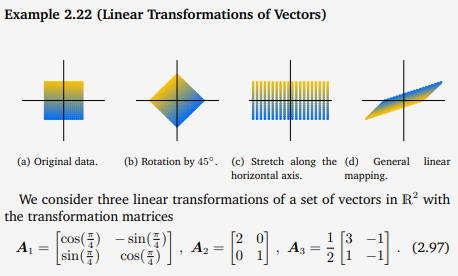
\includegraphics[width=12cm]{Mathematical Background/example-transformation-matrix-application.png}
\end{figure}\\
\textbf{Questions:}\\
%Where do the coefficients $\alpha_{ij}$ of the transformation matrix come from? Can we follow an example of calculating the transformation of one of the vectors from the image?
\subsubsection*{Basis Change}
In the following, we will have a closer look at ho w transformation matrices of linear mapping $\Phi: V \longrightarrow W$ change if we change the bases in V and W. Consider two ordered bases of V
\[ 
    B=(b_{1}, \ldots,b_{n}) \quad \tilde{B} = (\tilde{b}_{1}, \ldots,\tilde{b}_{n})
\]
and two ordered bases of W
\[ 
    C=(c_{1}, \ldots,c_{n}) \quad \tilde{C} = (\tilde{c}_{1}, \ldots,\tilde{c}_{n})
\]. Moreover, $A_\Phi \in \mathbb{R}^{m \times n}$ is the transformation matrix of the linear mapping $\Phi: V \longrightarrow W$ with respect to the bases B and C, and $\tilde{A}_\Phi \in \mathbb{R}^{m\times n}$ is the corresponding transformation mapping with respect to $\tilde{B} and \tilde{C}$. In the following we will investigate how $A$ and $\tilde{A}$ are related, for example how/whether we can transform $A_\Phi$ into $\tilde{A}_\Phi$ if we choose to perform a basis change from $B,C$ to $\tilde{B},\tilde{C}$.
\begin{theorem}[Basis Change]
    For a linear mapping $\Phi: V \longrightarrow W$, ordered bases of V
    \[ 
        B=(b_{1}, \ldots,b_{n}) \quad \tilde{B} = (\tilde{b}_{1}, \ldots,\tilde{b}_{n})
    \]and  of W
    \[ 
        C=(c_{1}, \ldots,c_{n}) \quad \tilde{C} = (\tilde{c}_{1}, \ldots,\tilde{c}_{n}) 
    \]
    and a transformation matrix $A_\Phi$ of $\Phi$ with respect to B and C, the corresponding transformation matrix $\tilde{A}\Phi$ with respect to the bases $\tilde{B} and \tilde{C}$ is given as 
    \[ 
        \tilde{A}_\Phi = T^{-1} A_\Phi S 
    \]
    Here, $S \in \mathbb{R}^{n\times n}$ is the transformation matrix of $id_V$ that maps coordinates with respect to $\tilde{B}$ onto coordinates with respect to B, and $T \in \mathbb{R}^{m\times m}$ is the transformation matrix of $id_W$ that maps coordinates with respect to $\tilde{C}$ onto coordinates with respect to C.
    \begin{figure}[htbp]
        \centering
        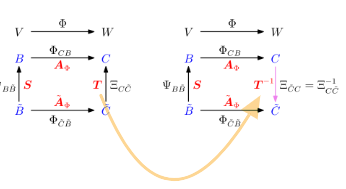
\includegraphics[width=8cm]{Mathematical Background/basischange.png}
    \end{figure}
\end{theorem}

\subsubsection*{Image and Kernel}
\begin{definition}[Image and Kernel]
    For $\Phi : V \rightarrow W$ we define the kernel/null space:
    \[ 
        ker(\Phi) := \Phi^{-1}(0_w) = {v \in V, \Phi(v) = 0_w} 
    \]and the image/range
    \[ 
         Im(\Phi) := \Phi(V) = \left\{ w \in W \mid \exists v \in V : \Phi(v) = w \right\}
    \]
    We also call V and W the domanin and codomain of $\Phi$ respectively.\\
    Intuitively, the kernel is the set of vectors $v\in V$ that $\Phi$ maps onto the neutral element $0_W \in W$. The image is the set of vectors $w \in W$ that can be "reached" by $\Phi$ from any vector in V.
    \begin{figure}[htbp]
        \centering
        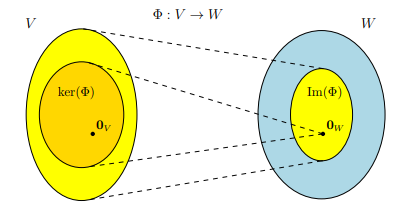
\includegraphics[width=8cm]{Mathematical Background/image-kernel.png}
    \end{figure}
\end{definition}
\begin{remark}[Null Space and Column Space]
    Let us consider $A \in \mathbb{R}^{m\times n}$ and a linear mapping $\Phi: \mathbb{R}^n \longrightarrow \mathbb{R}^m, \quad x \mapsto Ax$
    \begin{itemize}
        \item For $A=[a_{1}, \ldots,a_{n}]$, where $a_i$ are the columns of A, we obtain
        \[ 
            Im(\Phi) = {Ax: x \in \mathbb{R}^n} = \left\{ \sum_{i=1}^{n}{x_ia_i}:x_{1}, \ldots,x_{n}\in R \right\} = span[a_{1}, \ldots,a_{n}]\subseteq \mathbb{R}^m
        \]
    \end{itemize}
\end{remark}

\section*{Analytic Geometry}
In this chapter we will add some geometric interpretation and intuition to all of these concepts. In particular, we will look at geometric vectors and comput their lengths and distances or angle between two vectors. To be able to do this, we equip the vector space with an inner product that induces the geometry of the vector space.
\begin{figure}[htbp]
    \centering
    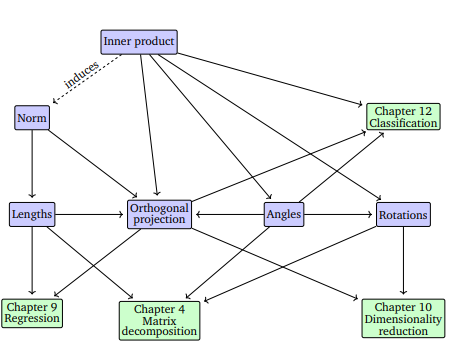
\includegraphics[width=11cm]{Analytical Geometry/mindmap.png}
\end{figure}
\subsection*{Norms}
\begin{definition}[Norm]
    A norm on a vector space V is a function 
    \begin{align*}
        \norm{\cdot}: &V \longrightarrow \mathbb{R}
        &x \mapsto \norm{x}
    \end{align*}
    which assigns each vector x its length $\norm{x} \in \mathbb{R}$, such that for all $\lambda \in \mathbb{R}$ and $x,y \in V$ the following hold: 
    \begin{itemize}
        \item Absolutely homogeneous: $\norm{\lambda x} = \absolute{\lambda}\norm{x}$
        \item Triangle inequality: $\norm{x+y} \leq \norm{x} + \norm{y}$
        \item Positive definite: $\norm{x} \geq 0$ an $\norm{x} = 0 \Longleftrightarrow x = 0$
    \end{itemize}
\end{definition}
The norm we will be using throughout these notes is going to be the Euclidean norm by default if not stated otherwise.
\begin{definition}[Euclidean Norm]
    The Euclidean norm of $x\in \mathbb{R}^n$ is defined as:
    \[ 
        \eunorm{x} = \sqrt[2]{\sum_{i=1}^{n}{x^2} = \sqrt{x^Tx}}
    \]and it computes the Euclidean distance from x to the origin. The Euclidean norm is also called the $\ell_2$ norm.
\end{definition}
\subsection*{Inner Products}
Recall the linear mappings where we can rearrange the mapping with respect to addition and multiplication with a scalar. A bilinear mapping $\Omega$ is a mapping with two arguments, and it is linear in each argument, i.e., when we look at a vector space V then it holds that for all $x,y,z \in V, \lambda, \psi \in \mathbb{R}$ that
\begin{align*}
    \Omega(\lambda x+ \psi y, z) = \lambda\Omega(x,y) + \psi\Omega(y,z)\\
    \Omega(x,\lambda y+ \psi z) = \lambda\Omega(x,y) + \psi \Omega(x,z)
\end{align*}
A bilinear mappings doesnt work on a single vector space but on the cartesian product of two vector spaces. We want to focus on biliear mappings that are: \begin{itemize}
    \item Symmetric: $\Omega(x,y)= \omega(y,x), \quad \forall x,y \in V$
    \item Positive definite: \[ 
        \forall x \in V\setminus\{0\} : \Omega(x,x) >0, \quad \Omega(\vec{0},\vec{0})= 0
    \]
\end{itemize}
\begin{definition}[Inner product]
    Let V be a vector space and $\Omega: V \times V \longrightarrow \mathbb{R}$ be a bilinear mapping that takes two vectors and maps them onto a real number. Then
    \begin{itemize}
        \item A positive definite, symmetric bilinear mapping $\Omega: V \times V \longrightarrow \mathbb{R}$ is called an inner product on V. We typically write $\anglepar{x,y}$ instead of $\Omega(x,y)$.
        \item The pair $(V,\anglepar{\cdot, \cdot})$ is called an inner product space or (real) vector space with inner product. If we use the dot product we call $(V,\anglepar{\cdot, \cdot})$ a Euclidean vector space. We will refer to these spaces as inner product spaces. 
    \end{itemize}
\end{definition}
Recall that any vectors $x,y \in V$ can be written as linear combinations of the basis vectors so that $x = \sum_{i=1}^{n}{\psi_i b_i} \in V$ and $y = \sum_{j=1}^{n}{\lambda_j b_j} \in V$ for suitable $\psi_i,\lambda_j \in \mathbb{R}$. Due to the bilinearity of the inner product, it holds for all $x,y \in V$ that
\[ 
    \anglepar{x,y} = \anglepar{\sum_{i=1}^{n}{\psi_ib_i}, \sum_{j=1}^{n}{\lambda_j b_j}} = \sum_{i=1}^{n}{\sum_{j=1}^{n}{\psi_i\anglepar{b_i,b_j}\lambda_j}} = \hat{x}A\hat{y}
\]where $A_{i,j} := \anglepar{b_i,b_j}$ and $\hat{x},\hat{y}$ are the coordinates of x and y with respect to the basis B. This implies that the inner product $\anglepar{\cdot, \cdot}$ is uniquely determined through A. The symmetry of the inner product also means that A is symmetric. Furthermore, the positive definiteness of the inner product implies that
\[ 
    \forall x \in V \setminus\{0\} : x^TAx>0
\]
\begin{definition}[Symmetric, Positive Definite Matrix]
    A symmetric matrix $A \in \mathbb{R}^{n\times n}$ that satisfies 
    \[ 
        \forall x \in V \setminus\{0\} : x^TAx>0 
    \]
    is called symmetric, positive definite or just positive definite. 
\end{definition}

\subsection*{Lengths and Distances}
\begin{remark}[Cauchy-Schwarz inequality]
    For an inner product vector space $(V, \anglepar{\cdot, \cdot})$ the induced norm $\norm{\cdot}$ satisfies the Cauchy-Schwarz inequality 
    \[ 
        \absolute{\anglepar{x,y}} \leq \norm{x}\norm{y} 
    \]
\end{remark}
\begin{definition}[Distance and Metric]
    Consider an inner product space $(V, \anglepar{\cdot, \cdot})$. Then 
    \[ 
        d(x,y):= \norm{x-y} = \sqrt{\anglepar{x-y,x-y}}
    \]is called the distance between x and y for $x,y \in V$. If we use the dot product as the inner product, then the distance is called Euclidean distance.\\
    The mapping
    \begin{align*}
        d: &V \times V \longrightarrow \mathbb{R}\\
        &(x,y) \mapsto d(x,y)
    \end{align*}
\end{definition}
A metric $d$ satisfies the following:
\begin{itemize}
    \item $d$ is positive definite, i.e., $d(x,y) \geq 0\; \forall x,y \in V$ and $d(x,y) = 0 \Longleftrightarrow x=y$
    \item $d$ is symmetric, i.e., $d(x,y) = d(x,y)\; \forall x,y \in V$
    \item Triangle inequality: $d(x,z) \leq d(x,y)+d(y,z) \; \forall x,y,z \in V$
\end{itemize}
\begin{remark}
    At first glance, the lists of properties of inner products and metrics look very similar. However, we observe that $\anglepar{x,y}$ and $d(x,y) $ behave in opposite directions. Very similar x and y will result in a large value for the inner product and a small value for the metric.
\end{remark}
\subsection*{Angles and Orthogonality}
In addition to enabling the definition of lenghts of vectors, as well as the distance between two vectors, inner products also capture the geometry of a vector space by defining the angle $\omega$ between two vectors. We use the Cauchy-Schwarz inequality to define angles $\omega$ in inner product spaces between two vectors x,y, and this notation coincides with our intuition in $\mathbb{R}^2$ and $\mathbb{R}^3$. Assume that $x \neq 0, y\neq 0$. Then 
\[ 
    -1 \leq \frac{\anglepar{x,y}}{\norm{x}\norm{y}} \leq 1 
\]
Therefore, there exists a unique $\omega \in [0,\pi]$ with 
\[ 
    \cos{\omega} = \frac{\anglepar{x,y}}{\norm{x}\norm{y}}
\]Intuitively, the angle between two vectors tells us how similar their orientations are.
\begin{definition}[Orthogonality]
    Two vectors $x$ and $y$ are orthogonal if and only if $\anglepar{x,y} = 0$ and we write $x \perp y$. If additionally $\norm{x} = 1 = \norm{y}$, the vectors x and y are orthonormal.
\end{definition}
\begin{definition}[Orthogonal Matrix]
    A square matrix $A \in \mathbb{R}^{n\times n}$ is an orthogonal matrix if and only if its columns are orthonormal so that 
    \[ 
        AA^T = I = A^TA 
    \]which implies that
    \[ 
        A^{-1} = A^T 
    \]
\end{definition}
\subsection*{Orthonormal Basis}
\begin{definition}[Orthonormal Basis]
    Consider an n-dimensional vector space V and a basis $b_{1}, \ldots,b_{n}$ of V. If 
    \begin{align*}
        \anglepar{b_i,b_j} = 0 \; for \; i\neq j \\
        \anglepar{b_i,b_j} = 1
    \end{align*}
    for all $i,j = 1, \ldots, n$ then the basis is called an orthonormal basis (ONB).
\end{definition}
\section{Tensor Flow}
Let's follow the computation of our program to recognise the 10 digits, our input matrix is $(1 \times 784)$, our weights matrix W $(784 \times 10)$ our bias matrix $(10 \times 1)$.\\
Matrix representation of neural networks:
\[ 
     L = XW + B
\]L = logits. These are the steps:\[ 
    Pr(A(x)) = \sigma(xW +b) 
\]
\[ 
    L(x) = -log(Pr(A(x)=a)) \quad \text{cross entrpy loss function}
\]
\[ 
    \nabla_l X(\Phi) = \left( \frac{\partial X(\Phi)}{\partial l_1}, \ldots, \frac{\partial X(\Phi)}{\partial l_m} \right) 
\]
\[ 
    \Delta W = -\mathcal{L}X^T\nabla_l X(\Phi) 
\]
Important we want to manipulate input in batches. Now the input matrix is now (m x 784), m batch size. When adding bias you might have to adjust the size of the matrix to work with the m rows of the batch input matrix. Tensor flow is the programming language and Python is the environment. Tensorflow plays with tensors (often typed). Vectors in Tensorflow only have one dimension! In the environment we set-up our nn-model by defining parameters and an architecture. We go trhough 3 stages: 
\begin{itemize}
    \item Create the tensors
    \item Turn them into a variable
    \item Initialize them
\end{itemize}
A tensorflow program:
\begin{itemize}
    \item Load data
    \item Set-up the model (batch-size)
    \item Learn the variables (parameters)
\end{itemize}
Along the way of training the model we must keep in mind to compute the accuracy.\\ Rule of thumb: the smaller the batch size the smaller the learning rate.\\
\subsection{Multilayered NNs}
Our model can work with multiple layered NNs but we cannot obtain any improvement if we don't include some non-linearity in the sense of an activation function on the neurons. We can clearly see it if we see that a one layer feed-forward NN is simply computing $y = XW$. If we add another layer of linear units U which feeds into a layer V:
\begin{align*}
    y &= (xU)V\\
    &= x(UV)
\end{align*}
Whatever capabilities captured in the two layers situation can be compacted in the single matrix $W = UV$.
Examples of activation functions are ReLU (rectified linear unity) and the Sigmoid. They are placed between the output of one layer and the input of the next one.\\
A key problem that we quickly encounter is the vanishing gradient that the ReLU solves better than the Sigmoid. Another improvement over the ReLU is the Leaky ReLU.
\[ 
    Pr(A(x)) = \underset{soft-max}{\sigma} (\underset{ReLU}{\rho}(xU+\underset{first-layer bias}{b_u})V+\underset{second-layer bias}{b_v}) 
\]


\section{Learning Paradigms and Terminology}
In describing the learning paradigms and the terminology we must keep in mind an objective: to be able to generalize the concepts observed.
\begin{definition}[Neural Network]
    A neural network is a sorted triple $(N,V,w)$ with two sets $N,V$ and a function w, where N is the set of neurons and V is a set ${(i,j)|i,j\in\mathbb{N}}$ whose elements are connections between neurons. The function $w: V \longrightarrow \mathbb{R}$ defines the weights where $w((i,j))$, the weight between neuron i and j, is shortened $w_{i,j}$
\end{definition}
The data flow is more than just a graph: data enters a neuron where it follows three steps:
\begin{description}
    \item[Propagation function] Often a weighted sum, transforms outputs of other neurons to net input
    \item[Activation function] Transforms net input and sometimes old activation to new activation
    \item[Output function] Often the identity function, transforms activation to output for other neurons
\end{description}
\begin{definition}[Propagation function and network input]
    Let $I = \left\{ i_{1}, \ldots,i_{n} \right\}$ be the set of neurons such that $\forall z\in \left\{ 1, \ldots, n \right\} : \exists w_{i_z,j}$. Then the network input of j, called $net_j$, is calculated by the propagation function $f_prop$ as follows
    \[ 
        net_j = f_prop(o_{i_1},\ldots, o_{i_n}, w_{i_1,j} \ldots w_{i_n,j}) 
    \]
    Most often the $f_prop$ is the weighted sum and operates on previous layers' output
\end{definition}
\begin{definition}[Threshold value]
    Let j be a neuron. The threshold value $\Theta_j$ is uniquely assigned to j and marks the position of the maximum gradient value of the avtivation function.
\end{definition}

\begin{definition}[Activation state/ activation in general] Let j be a neuron. The activation state $a_j$, in short activation, is explicitly assigned to j, indicates the extent of the neurons activity and results from the activation function.
    \[ 
        a_j(t) = f_act(net_j(t), a_j(t-1), \Theta_j) 
    \]
    
\end{definition}
Most often, the output function is the identity function. Unlike the other variables within the neural network the activation functions is often defined globally for all neurons, or at least for a set of neurons and only the threshold values are different for each neurons. The following are commong activation functions:
\begin{figure}[htbp]
    \centering
    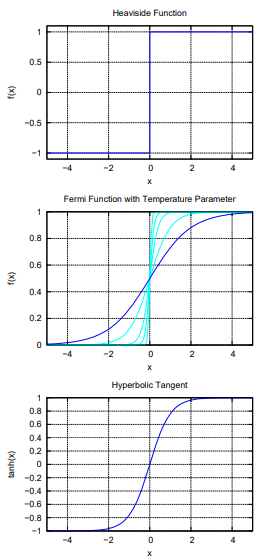
\includegraphics[width=8cm]{Learning Paradigms/activation_functions.png}
\end{figure}
\newpage
\begin{definition}[Output function]
    Let j be a neuron. The output function
    \[ 
        f_out(a_j)= o_j 
    \]
    calculates the output value of $o_j$ of the neuron j from its avtivation state $a_j$.
\end{definition}
    Generally the output function is defined globally. Often this function is the identity function $f_out(a_j) = a_j,\; o_j = a_j$
\begin{definition}[Bias neuron]
    A bias neuron is a neuron whose output value is always 1. It is used to represent neuron biases as connection weights, which enables any weight training algorithm to train the biases at the same time.
\end{definition}
\subsection{Network Topologies}
\subsubsection{Feed-Forward}
The Feed-forward network topology has input nodes, hidden/processing nodes, and output nodes. Most often layers are fully connected. They can be varied adding shortcuts between input and output cutting through the network while in the simplest topology each neuron is only connected to neurons of the adjacent layer.
\begin{figure}[htbp]
    \hspace*{-2cm}
    \centering
    \begin{subfigure}{8cm}
      \centering
      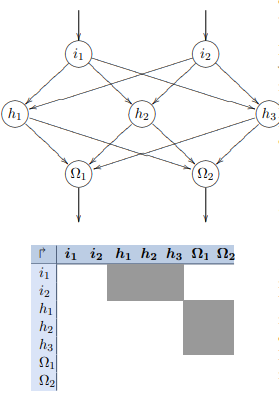
\includegraphics[width=6cm]{Learning Paradigms/simplest_ffnn.png}
      \caption{Simplest Feed-forward NN}
      \label{fig:sub1}
    \end{subfigure}%
    \begin{subfigure}{8cm}
      \centering
      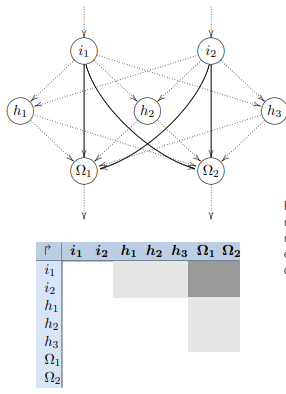
\includegraphics[width =6cm]{Learning Paradigms/shortcut_ffnn.png}
      \caption{Feed-forward NN with shortcuts}
      \label{fig:sub2}
    \end{subfigure}
    \caption{Feed-forward topologies}
    \label{fig:feedforward}
    \end{figure}
\subsubsection{Recurrent}
By recurrence in the context of NN we mean the process of a neuron influencing itself by any means or by any connection.
In recurrent NN it's not as clear what neurons are the outputs. The use and impact of recurrence in neural networks is extremely complex and is still being researched. Recurrence can be of three types: direct (self loop), indirect, lateral.
\begin{figure}[htbp]
    \centering
    \begin{subfigure}{6cm}
      \centering
      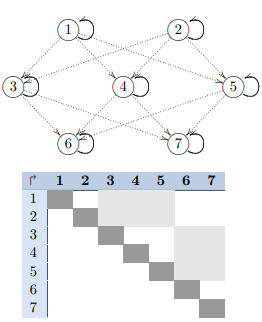
\includegraphics[width=5cm]{Learning Paradigms/direct_recurrence.png}
      \caption{Direct recurrence}
      \label{fig:sub1}
    \end{subfigure}%
    \begin{subfigure}{6cm}
      \centering
      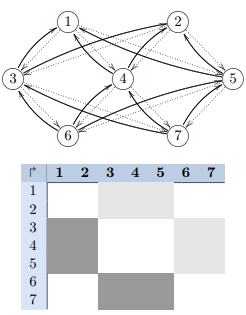
\includegraphics[width =5cm]{Learning Paradigms/indirect_recurrence.png}
      \caption{Indirect recurrence}
      \label{fig:sub2}
    \end{subfigure}
    \begin{subfigure}{6cm}
        \centering
        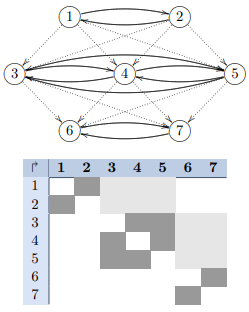
\includegraphics[width =5cm]{Learning Paradigms/lateral_recurrence.png}
        \caption{Lateral recurrence}
        \label{fig:sub3}
      \end{subfigure}
    \caption{Recurrence in NN}
    \label{fig:recurrence}
    \end{figure}
\subsection{Order of activation}
To describe the order of activation we have two classes:
\begin{description}
    \item[Synchronous activation]: all neurons change their values synchronously ( they simultaneusly calculate network input, activation and output, and pass them on). The syncronous activation corresponds closest to its biology counterpart but not particularly effective for real world hardware, especially if used on Feed-forward NN.
    \item[Asynchronous activation]: here, the neurons do not change their values simultaneusly but at different points of time. For this, there exist different orderds:
    \begin{description}
        \item[Random Order] a random neuron i is chosen and its $net_i, a_i, o_i$ are updated. For n neurons a cycle is the n-fold execution of this step. Some neurons might be updated more than once and other never.
        \item[Random Permutation] in this case each neuron is chosen exactly once but in a random order, during one cycle.
        \item[Topological Order] the neurons are updated during one cycle and according to a fixed order. The order is defined by network topology. 
    \end{description} 
\end{description}
\begin{definition}[Input Vector]
    A network with n input neurons needs n inputs $x_{1}, \ldots,x_{n}$. They are considered as input vecotr $ x = (x_{1}, \ldots,x_{n})$. As a consequence the input dimension is referred to as n.
\end{definition}
\begin{definition}[Output Vector]
    A network with m output neurons provides m outputs $y_{1}, \ldots,y_{n}$. They are considered as output vecotr $ y = (y_{1}, \ldots,y_{n})$. As a consequence the output dimension is referred to as m.
\end{definition}

\subsection*{Learnin paradigms}
How do we act on a NN to improve its ability towards generalization? There are at least 7 actions that we can take:
\begin{itemize}
    \item developing new connections
    \item deleting existing connections
    \item changing connecting weights
    \item changing the threshold values of neurons
    \item varying one or more of the three neuron functions
    \item developing new neurons
    \item deleting existing neurons (and of course connections)
\end{itemize}
\begin{definition}[Training set]
    A training set (named P) is a set of training patterns $p_{1}, \ldots,p_{n}$, which we use to train our neural net. 
\end{definition}
Two questions quickly arise when thinking about the network's ability to learn 
\begin{itemize}
    \item How do NNs learn?
    \item When do NNs stop learning?
\end{itemize}
There are three essential paradigms of learning by presenting the differences between their training set.
Unsupervised learning is the biologically most plausible method, but is not suitable for all problems. Only the input patterns are given; the network tries to identify similar patterns and to classify them into similar categories.
\begin{definition}[Unsupervised Learning]
    The training set only consists of input patterns, the network tries by itself to detect similarities and to generate pattern classes.
\end{definition}
In reinforcement learning the network receives a logical or a real value after completion of a sequence, which defines whether the result is right or wrong. Intuitively it is clear that this procedure should be more effective than unsupervised learning since the network receives specific criteria for problem-solving.
\begin{definition}[Reinforcement Learning]
    The training set consists of input patterns, after completion of a sequence a value is returned to the network indicating whether the result was right or wrong and, possibly, how right or wrong it was.
\end{definition}
In supervised learning the training set consists of input patterns as well as their correct results in the form of the precise activation of all output neurons. Thus, for each training set that is fed into the network the output, for instance, can directly be compared with the correct solution and the network weights can be changed according to their difference.
\begin{definition}[Supervised Learning]
    The training set consists of input patterns with correct results so that the network a precise error vector can be returned.
\end{definition}
\begin{definition}[Offline learning]
    Several training patterns are entered into the network at once, the errors are accumulated and it learns for all patterns at the same time.
\end{definition}
\begin{definition}[Online learning]
    The network learns directly from the errors of each training sample.
\end{definition}
\subsection{Learning curve and error measurement}
\begin{definition}[Training patterns]
    A training pattern is an input vector p with the components $p_{1}, \ldots,p_{n}$ whose desired output is known. By entering the training pattern into the network we receive an output that can be compared with the teaching input, which is the desired output. The set of training patterns is called P. It contains a finite number of ordered pair (p, t) of training patterns with corresponding desired output.
\end{definition}
\begin{definition}[Teaching Input]
    Let j be an output neuron. The teaching input $t_j$ is the desired and correct value j should output after the input of a certain training pattern. Analogously to the vector p the teaching inputs $t_{1}, \ldots,t_{n}$ of the neurons can also be combined into a vector $t$. $t$ always refers to a specific training pattern $p$ and is, as already mentioned, contained in the set P of the training patterns.
\end{definition}
\begin{definition}[Error Vector]
    For serveral output neurons $\Omega_{1}, \ldots,\Omega_{n}$ the difference between output vector and teaching input under a training input p
    \[ 
        E_p = \begin{bmatrix}
            t_1-y_1 \\
            \vdots\\
            t_n-y_n
        \end{bmatrix} 
    \]is referred to as error vector. 
\end{definition}
The learning curve indicates the progress of the error, which can be determined in various ways.
\begin{definition}[Specific Error]
    The specific error $Err_p$ is based on a single training sample, which means it is generated online.\\
    Additionally, the Root Mean Square and the Euclidean Distance are often used.
\end{definition}
\begin{definition}[Total Error]
    The total error $Err$ is based on all training samples, that means it is generated offline.
\end{definition}

\section{Convolutional Neural Networks}

The goal is to analyse the relationship and the overlap between the terms kernel, filters and convolution. Question: why should we have each computing unit from one layer completely connected to every other computing unit to the next one?\\
Convolutional neural networks are one example of partially connected neural netoworks and are best introduced when discussing applications related to vision.\\
When thinking about solving visual problems such as scene recognition the focus is on the difference in pixel values, not their absolute values. In convolutional neural networks we use filters (convolutional filters and kernel filter) to determine and hightlight such differences. A filter is a window, typically pretty small, that slides over an image. A filter highlights differences present in the data wherever the pattern filtered is encountered. We convolve a filter with a patch of an image, this way we get that we convolve a filter with an image. Formally a convolution is a computation of a generalized dot product.
\begin{definition}[Kernel Function]
    We consider the convolution kernel to be a function, the kernel function. We get the value V of this function at a position x,y on an image I as follows:
    \[ 
        V(x,y) = (I\cdot K) (x,y) = \sum_{m}{\sum_{n}{I(x+m,y+n)K(m,n)}}
    \]
\end{definition}
Key point: where do we get the values for a filter? Before deep learning they were thoughtfully crafted but now these are parameters that we can learn.
\subsection{The architecture of convolutional neural networks}
Usually we have a lot of different filters and the goal of each filter is to pick up a specific feature in the image. We can refer to this set of filters a bank of filter. The architecture of a convolutional neural networks takes the output of the bank of filters step and feeds it through a standard fully connected layer followed by a softmax. A convolutional filter bank is at least a three-dimensional tensor in which the dimensions are height, width and number of channels. 
\begin{definition}[Stride]
    Stride can be vertical and horizontal and is defined as the number of cells to move before applying again the filter.\\Furthermore the stride can be of tipe Valid or Same: the first kind reduces the input sizes (most of the times), same maintains size (with stride 1). 
\end{definition}
\section{Math}
\subsection{Projections}
Projections are an important class of linear transformation. When we compress of visualize high-dimensionality data, we will lose information. To minimize this compression loss, we ideally find the most informative dimensions in the data.
\begin{definition}[Projection]
    Let V be a vector space $U \subseteq V$ a subspace of V. A linear mapping $\pi: V \longrightarrow U$ is called a projection if $\pi^2 = \pi \circ \pi = \pi$.
\end{definition}
A projection, in general, means concentrating on a particular direction, feature, set of features. Since the projection $\pi$ is a linear mapping and they can be expressed by transformation matrix there esists a transformation matrix $P_\pi$ such that $ P_\pi^2 = P_\pi $
\subsubsection{Projection onto one-dimensional subspaces}
\begin{definition}[Projection onto one-dimensional subspaces (lines)]
    Assume we are given a line (a one-dimensional subspace) through the origin with basis vector $b\in \mathbb{R}^n$. The line is a one-dimensional subspace $U\subseteq \mathbb{R}^n$ spanned by b. When we project $x \in \mathbb{R}^2$ onto U, we seek the vector $\pi_U(x) \in U$ that is closest to x. 
\end{definition}
\begin{figure}[htbp]
    \centering
    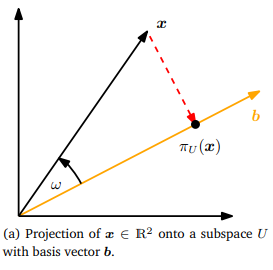
\includegraphics[width = 7cm]{Math/projectin_onto_line.png}
\end{figure}
Properties of the projection $\pi_U(x)$:
\begin{itemize}
    \item The projection $\pi_U(x)$ is closest to x, where "closest" implies that the distance $ \norm{vec x - \pi_u(vec x)} $ is minimal. It follows that the segment $\pi_U(x) -x$ from $\pi_U(x)$ to x is orthogonal to U, and therefore the basis vector b of U.
    \item The projection $\pi_U(x)$ of x onto U must be an element of U and, thereforre, a multiple of the basis vector b that spans U. Hence, $\pi_U(x) = \lambda b$, for some $\lambda \in \mathbb{R}$.
\end{itemize}
In the following three steps, we determine the coordinate $\lambda$, the projection $\pi_u(x) \in U$ and the projection matrix $P_\pi$ that maps any $x \in \mathbb{R}^n$ onto U.
\begin{enumerate}
    \item Finding the coordinate lambda. The orthogonality condicion yields
    \[ 
        \anglepar{x-\pi_U(x),b}= 0 \overset{\pi_U(x)=\lambda b}{\Longleftrightarrow } \anglepar{x-\lambda b, b} = 0
    \]We can now exploit the bilinearity of the inner product and arrive at
    \[ 
        \anglepar{x,b} -\lambda \anglepar{b,b}=0 \Longleftrightarrow \lambda = \frac{\anglepar{x,b}}{\anglepar{b,b}} = \frac{\anglepar{b,x}}{\norm{b}^2} 
    \]In the last step, we exploited the fact that inner products are symmetric. If we chose $\anglepar{\cdot,\cdot}$ to be the dot product, we obtain
    \[ 
        \lambda = \frac{b^Tx}{b^tb}= \frac{b^Tx}{\norm{b}^2} 
    \]If $\norm{b}=1$, then the coordinate $\lambda$ of the projection is given by $b^Tx$.
    
    \item Second step is always easy $ \pi_U(x) = \lambda b = \frac{\anglepar{x,b}}{\norm{b}^2}b = \frac{b^tx}{\norm{b}^2}b $ 
    \item Just rewrite to determine a matrix such that $ \pi_U(x) = P_\pi x$ we see that $P = \frac{b b^T}{\norm{b}^2} $ 
\end{enumerate}
\subsubsection{Projection onto general subspaces}
In the following we look at orthogonal projections of vectors $x \in \mathbb{R}^n$ onto lower-dimensional subspaces $U\subseteq \mathbb{R}^n$ with $\dim(U) = m \geq 1$. Assume that $(b_{1}, \ldots,b_{m})$ is an ordered basis of U. As for the one-dimensional case, we follow a three-step procedure. 
\begin{enumerate}
    \item Find the coordinates $\lambda_{1}, \ldots,\lambda_{m}$ of the projection (with respect to the basis of U), such that the linear combination
    \begin{align*}
        \pi_U(x) = \sum_{i=1}^{m}{\lambda_ib_i= B\lambda}\\
        B = [b_{1}, \ldots,b_{m}] \in \mathbb{R}^{n\times m}, \quad \lambda = [\lambda_{1}, \ldots,\lambda_{m}]^T \in \mathbb{R}^m
    \end{align*}
    is closest to $x \in \mathbb{R}^n$. Again, closest refers to minimum distance which means that the vector connecting $\pi_U(x) \in U$ and $x\in \mathbb{R}^n$ must be orthogonal to all basis vectors of U.
    After some more considerations we get the normal equation $\lambda = (B^TB)^{-1}B^Tx$, where $(B^TB)^{-1}B^T$ is called the psuedo inverse of B (which is not square). It can always be computed if BTB is invertible, this is true since B is a basis for U.
    \item Find the projection $\pi_U(x) \in U$ We already established that $\pi_U(x)=B\lambda$. Therefore
    \[ 
        \pi_U(x) = B(B^TB)^{-1} 
    \]
    \item Find the projection matrix $P_\pi$. From 2 we can immediately see that the projection matrix that solves $P_\pi x=\pi_U(x)$ must be 
    \[ 
        P_\pi=B(B^TB)^{-1}B^T 
    \]
\end{enumerate}
Projection is a tool for finding approximate solutions (by deleting some solutions). Projecting is easier when the base is orthonormal because BTB = I. Through Gram-Schmidt Orthogonalization we can turn any basis into an orthonormal one, going one dimension at a time.

\subsection{Matrix Decomposition}
\begin{figure}[htbp]
    \centering
    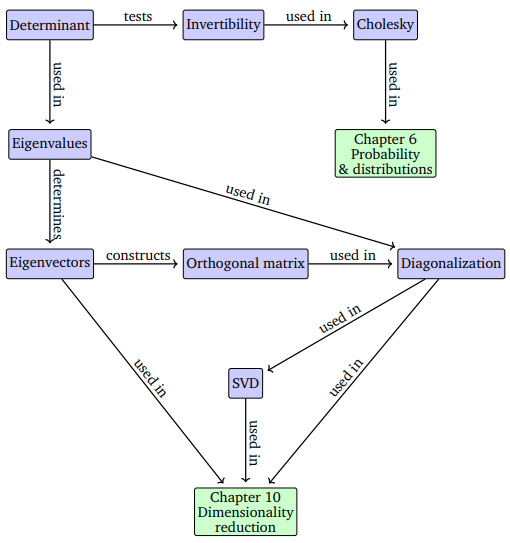
\includegraphics[width=10cm]{Math/matrix-decomposition-map.png}
\end{figure}
\subsubsection{Determinant and Trace}
The determinant of a square matrix A is a function that sends the matrix to a real number. A square matrix A is invertible if and only if $\det(A)= 0$ , this means that $rk(A)=n$. Two vectors in $\mathbb{R}^2$ are linearly independent if and only if they form a proper parallelogram.
\begin{theorem}[Laplace Expansion]
    Consider a matrix $A \in \mathbb{R}^{n\times n}$. Then, for all $j = 1, \ldots,n$:
    \begin{enumerate}
        \item Expansion along column j
        \[  
            \det(A) = \sum_{k=1}^{n}{(-1)^{k+j}a_{kj}\det(A{k,j})}  
        \]
        \item Expansion along row j
        \[  
            \det(A) = \sum_{k=1}^{n}{(-1)^{k+j}a_{jk}\det(A{j,k})}  
        \]
    \end{enumerate}
    Here $A_{k,j} \in \mathbb{R}^{(n-1)\times (n-1)}$ is the submatrix of A that we obtain when deleting row k and column j.
\end{theorem}
For $n=3$ the Sarrus'rule helps us calculate the determinant:
\begin{align*}
    \begin{bmatrix}
        a_{11} & a_{12} &a_{13}\\
        a_{21} & a_{22} &a_{23}\\
        a_{31} & a_{32} &a_{33}
    \end{bmatrix} &= a_{11}a_{22}a_{33}+a_{21}a_{32}a_{13}+a_{31}a_{12}a_{23}\\
    &-a_{31}a_{22}a_{13}-a_{11}a_{32}a_{23}-a_{21}a_{12}a_{33}
\end{align*}
For a triangular matrix $T \in \mathbb{R}^{n\times n}$, the determinant is the product of the diagonal elements
\[ 
    \det(T) = \Pi_{i=1}^{n}{T_{ii}} 
\]
The following are some of the properties of determinants:
\begin{itemize}
    \item The determinant of a matrix product is the product of the corresponding determinants, $\det(AB) = \det(A)\det(B)$
    \item Determinants are invariant to transposition, $det(A) = det(A^T)$
    \item If A is regular (invertible), then $\det(A^{-1})= \frac{1}{\det(A)}$
    \item Similar matrices possess the same determinant and the determinant is invariant to the choice of basis for the linear mapping
    \item Adding a multiple of a column/row to another one does not change $\det(A)$
    \item Swapping two rows/columns changes the sign of the determinant
\end{itemize}
\begin{definition}[Trace of a matrix]
    The trace of a square matrix $A \in \mathbb{R}^{n\times n}$ is defined as
    \[ 
        tr(A) = \sum_{i=1}^{n}{a_{ii}} 
    \]
    the trace is the sum of the diagonal elements of A and it satisfies the following properties:
    \begin{itemize}
        \item $tr(A+B) = tr(A) + tr(B), \quad A, B \in \mathbb{R}^{n\times n}$
        \item $tr(\alpha A) = \alpha tr(A)$
        \item $tr(I_n) = n$
        \item $tr(AB) = tr(BA), \quad A \in \mathbb{R}^{n\times k}, B \in \mathbb{R}^{k\times n}$
    \end{itemize}
\end{definition}
\begin{definition}[Characteristic Polynomial]
    For $\lambda \in \mathbb{R}$ and a square matrix $A \in \mathbb{R}^{n \times n}$
    \begin{align*}
        p_A(\lambda)&:= \det(A-\lambda I)\\
        & c_0 + c_1\lambda + c_2\lambda^2+ \cdots + c_{n-1}\lambda^{n-1}+(-1)^n\lambda ^n
    \end{align*}
    $c_{1}, \ldots,c_{n-1} \in \mathbb{R}$, is the characteristic polynomial of A. In particular
    \begin{align*}
        c_0 & = \det(A)\\
        c_{n-1} & = (-1)^{n-1} tr(A)
    \end{align*}
\end{definition}
\subsubsection{Eigenvalues and Eigenvector}
\begin{definition}[Eigenvalue and Eigenvector]
    Let $ A \in \mathbb{R}^{n\times n}$ be a square matrix. Then $\lambda \in \mathbb{R}$ is an eigenvalue of A and $x\in \mathbb{R}^n\setminus{0}$ is the corresponding eigenvector of A if
    \[ 
        Ax = \lambda x 
    \]
    We refer to this equation as the eigenvalue equation.
\end{definition}
\begin{theorem}
    $\lambda in \mathbb{R}$ is an eigenvalue of $A \in \mathbb{R}^{n\times n}$ if and only if $\lambda$ is a root of the characteristic polynomial $p_A(\lambda)$ of A.
\end{theorem}
\begin{definition}[Algebraic multiplicity]
    Let a square matrix A have an eigenvalue $\lambda_i$. The algebraic multiplicity of $\lambda_i$ is the number of times the root appears in the characteristic polynomial. 
\end{definition}
\begin{definition}[Eigenspace and Eigenspectrum]
    For $A \in \mathbb{R}^{n \times n}$ the set of all eigenvectors of A associated with an eigenvalue $\lambda$ spans a subspace of $\mathbb{R}^n$, which is called the eigenspace of A with respect to $\lambda$ and is denoted by $E_\lambda$. The set of all eigenvalues of A is called the eigenspectrum, or just spectrum, of A
\end{definition}
\begin{definition}[Geometric multiplicity]
    Let $\lambda_i$ be an eigenvalue of a square matrix A. Then the geometric multiplicity of $\lambda_i$ is the number of linearly independent eigenvectors associated with $lambda_i$. In other words, it is the dimensionality of the eigenspace spanned by the eigenvectors associated with $\lambda_i$. 
\end{definition}
\section{Learning}
Many questions related to learning from a mathematical standpoint:
\begin{itemize}
    \item What if we do not have a direct (e.g. visual) way to find the features?
    \item What if we want to know when to stop learning?
\end{itemize}
Using the papaya example we want to define learning. Learning means to produce a predictor/classifier/hypothesis that best approximates $f$ which is the "correct" labeling function. 
\[ 
    h: \mathcal{X} \longrightarrow \mathcal{Y}
\]using an algorithm $A(S)$ called the learning algorithm.
Here A is an algorithm, in the following $A\subseteq \mathcal{X}$
\subsection{Data}
We do not have access to the whole $\mathcal{X}$ so our data is given to us from a probability distribution. $\mathcal{D}$ is the probability distribution of $\mathcal{X}$. Also the truth function is a function from the domain to the codomain, and it's the correct classifier
\[ 
    f: \mathcal{X} \longrightarrow \mathcal{Y} 
\].
On these grounds we can introduce a measure (of the error) to compare $h$ and $f$. How do we single out the measure? 
\begin{enumerate}
    \item Get $A \subseteq \mathcal{X}$
    \item Determine how likely is to pick an x with distribution $\mathcal{D}$ and to fall in A: $\mathcal{D}(A)$
    \item In order to do step 2, we use the characteristic function of A
    \[ 
        \pi_A : \mathcal{X} \longrightarrow \{0,1\}\quad A = {x\in \mathcal{X}\mid \pi_A(x)=1} 
    \]
\end{enumerate}
Putting together step 2 and 3 we can use the following notation to express $\mathcal{D}(A)$ :
\[ 
    \mathbb{P}_{x\sim\mathcal{D}}[\pi(x)=1] = \mathcal{D(A)} 
\]
We define the error of a prediction rule as $h: \mathcal{X}\longrightarrow \mathcal{Y}$:
\[ 
    L_{\mathcal{D},f}(h)= \mathbb{P}_{x\sim D}[h(x)\neq f(x)]=\mathcal{D}(\left\{ x: h(x) \neq f(x) \right\}) 
\]$\mathcal{D} $ and $f$ are our assumptions and together with the definition of loss we established we have a measure of the true loss of the learner. In practice, though, we only have S and on its domain we consided $h$ and 
\[ 
    L_S(h) = \frac{\absolute{\left\{ i \in[m]: h(x_i) \neq y_i \right\}}}{m} 
\]
This is the empirical error and the practice of focusing and using it instead of the true error is called empirical risk minimization (ERM).
\subsection{Overfitting}
We now have the tools to illustrate overfitting very clearly:
\[ 
    h_S(x) = \begin{cases}
        y_i & if\; \exists i \in [m]\; s.t. \; x_i = x\\
        0 & otherwise
    \end{cases} 
\]It performs perfectly on S but might have much bigger error on the whole $\mathcal{X}$
\[ 
    \underset{estim. error}{L_S(h_S) = 0} \quad \underset{true error}{L_{\mathcal{D},f}(h_S)= \frac{1}{2}} 
\]
The cure for overfitting is to choose in advance, before seeing the data, a set of predictors. This set is called a hypothesis class and it's denoted by $\mathcal{H}$. For a given class $\mathcal{H}$, and a training sample, S, the $ERM_\mathcal{H}$ learner uses the ERM rule to choose a predictor, $h \in \mathcal{H}$, with the lowest possible error over S
\[ 
    ERM_\mathcal{H}(S) \in argmin_{h \in \mathcal{H}}{L_S(h)} 
\]
By restricting the learner to choosing a predictor from $\mathcal{H}$, we bias it toward a particular set of predictors. Such restrictions are referred to as inductive bias. 
The fundamental question is over which hypothesis classes $ERM_\mathcal{H}$ we don't end up overfitting. Intuitively, choosing a more restricted hypothesis class better protects us against overfitting but at the same time might cause us a stronger inductive bias. 
\subsubsection{Finite Hypothesis Classes}
The simplest type of restriction on a class is imposing an upper bound on its size. Here we show that if $\mathcal{H}$ is a finite class then $ERM_\mathcal{H}$ will not overfit, provided it is based on a sufficiently large training sample. 
\begin{definition}[The realizabiliity assumption]
    There exists $h^* \in \mathcal{H}$ such that $L_{\mathcal{D},f} (h^*) = 0$. Note that this assumption implies that with probability 1 over random samples, S, where the instances of S are sampled according to $\mathcal{D}$ and are labeled by f, we have $L_S(h^*) = 0$.
\end{definition}
We are making another important assumption: that all the examples in the trainin set S are independently and identically distributed (i.i.d.) according to the distribution $\mathcal{D}$ and labeled according to $f$. We denote this assumption by $S \sim \mathcal{D}^m$ where m is the size of S. We can see the training set S as a window over the distribution $\mathcal{D}$ and the function $f$, the larger the window the more likely it is to reflect more accurately the distribution and labeling used to generate it.\\
If S is chosen randomly we can see that a "wrong" choice leads to a "wrong" result, for this reason we need an estimate of the probability of picking the "wrong" S. The probability of picking a non-representative S is $\delta$, while we refer to $(1-\delta)$ as the confidence parameter of our prediction. \\We cannot guarantee a perfect label prediction, so we introduce an accuracy parameter and we interpret a measure of our accuracy parameter larger than some treshold $\epsilon$ as a failure by the learner.
Therefore we are interesting in upper bounding the probability to sample m-tuple of instances that will lead to failure of the learner. Formally, let $S\mid_x = (x_{1}, \ldots,x_{m})$ be the instances of the training set. We want to upper bound the probability of picking a bad $S\rvert_x$ for the ERM $h_S$.
\[ 
    \mathcal{D}^m\left( \left\{ S\rvert_x : L_{\mathcal{D},f}(h_S)>\epsilon \right\} \right) 
\]
Let $\mathcal{H}_B$ be the set of "bad" hypotheses, that is,
\[ 
    \mathcal{H}_B = \left\{ h \in \mathcal{H}: L_{\mathcal{D},f}(h)>\epsilon \wedge L_S(h)=0 \right\} 
\]In addition let
\[ 
    M = \left\{ S\rvert_x : \exists h \in \mathcal{H}_B, L_S(h)= 0 \right\}
\]be the set of misleading samples and it't what we want to bound. Since the realizabiliity assumption implies that $L_S(h_S)=0$, it follows that the event $L_{\mathcal{D},S}(h_S)>\epsilon$ can only happen if for some $h\in \mathcal{H}_B$ we have that $L_S(h) =0$. In other words, this event will only happen if our sample is in the set of misleading samples M. We can rewrite M as
\[ 
    M = \bigcup_{h\in\mathcal{H}_B}\left\{ S\rvert_x : L_S(h) = 0 \right\} 
\]
Hence,
\[ 
    D^m(\left\{ S\rvert_x:L_{\mathcal{D},f}(h_S) > \epsilon \right\})\leq D^m(M) = D^m(\cup_{h\in\mathcal{H}_B}\left\{ S\rvert_x : L_S(h) =0 \right\}) 
\]
We upper bound the right-hand of the preceding equation using the union bound, a basic property of probabilities.
\[ 
    \mathcal{D}(A \cup B ) \leq \mathcal{D}(A)+\mathcal{D}(B) 
\]Applying the union bound to the right-hand side of the equation yields:
\begin{equation}
    \mathcal{D}^m(\left\{ S\rvert_x: L_{\mathcal{D},f}(h_s)>\epsilon \right\})\leq \sum_{h\in\mathcal{H}_B}{\mathcal{D}^m(\left\{ S\rvert_x : L_S(h) = 0 \right\})}
\end{equation}
Next, let us bound each summand of the right-hand side of the preceding inequality. Fix some "bad" hypothesis $h \in \mathcal{H}_B$. The event $L_S(h) = 0$ is equivalent to the event $\forall i, h(x_i) = f(x_i)$. Since the examples in the trainin set are sampled i.i.d. we get that
\begin{align*}
    \mathcal{D}^m(\left\{ S\rvert_x : L_S(h) = 0 \right\}) &= \mathcal{D}^m(\left\{ S\rvert_x : \forall i,h(x_i) = f(x_i) \right\})\\
    & = \Pi_{i=1}^{m}{\mathcal{D}(\left\{ x_i: h(x_i) = f(x_i) \right\})}
\end{align*}
For each individual sampling of an element of the training set we have
\[ 
    \mathcal{D}({x_i:h(x_i) = y_i}) =1 - L_{\mathcal{D},f}(h) \leq 1-\epsilon
\]
where the last inequality follows from the fact that $h\in \mathcal{H}_B$. Combining the two previous equation and the inequality $1-\epsilon \leq e^{-\epsilon}$ we obtain that for every $h\in\mathcal{H}_B$
\[ 
    \mathcal{D}^m(\left\{ S\rvert_x : L_S(h) = 0 \right\}) \leq (1-\epsilon)^m \leq e^{-\epsilon m}
\]Combining this equation with ... we conclude that
\[ 
    \mathcal{D}^m(\left\{ S\rvert_x : L_{\mathcal{D},f}(h_S) > \epsilon \right\}) \leq \absolute{\mathcal{H}_B}e^{-\epsilon m}\leq \absolute{\mathcal{H}}e^{-\epsilon m}
\]
\begin{corollary}
    Let $\mathcal{H}$ be a finite hypothesis class. Let $\delta \in (0,1), \epsilon >0$ and let m be an integer that satisfies
    \[ 
        m\geq \frac{\log(\absolute{\mathcal{H}}/\delta)}{\epsilon} 
    \]
    Then fory labeling function f and for any distribution $\mathcal{D}$, for which the realizabiliity assumption holds, with probability of at least $1-\delta$ over the choice of an i.i.d. sample S of size m, we have that for every ERM hypothesis $h_S$ it holds that
    \[ 
        L_{\mathcal{D},f}(h_S) \leq \epsilon 
    \]
\end{corollary}
The preceding corollary tells us that for a sufficiently large m, the $ERM_{\mathcal{H}}$ rule over a finite hypothesis class will be \textbf{probably} (with confidence $1-\delta$) \textbf{approximately} (up to an error of $\epsilon$) \textbf{correct}. This model is called PAC learning. 
\begin{definition}(PAC learnability)
    A hypothesis class $\mathcal{H}$ is PAC learnable if there exists a function $m_{\mathcal{H}}:(0,1)^2 \longrightarrow \mathbb{N}$ and a learning algorithm with the following property: For every $\epsilon, \delta \in (0,1)$, for every distribution $\mathcal{D}$ over $\mathcal{X}$, and for every labeling function $f: \mathcal{X}\longrightarrow\left\{ 0,1 \right\}$, if the realizable assumptino holds with respect to $\mathcal{H}, \mathcal{D}, f$, then when running the learning algorithm on $m \geq m_{\mathcal{H}}(\epsilon, \delta)$ i.i.d. examples generated by $\mathcal{D}$ and labeled by $f$, the algorithm returns a hypothesis $h$ such that, with probability of at least $1-\delta$ (over the choice of the examples), $L_{\mathcal{D},f}(h)\leq \epsilon$
\end{definition}
\section{Word Embeddings}
 When introducing the concept of word embeddings we can say that our aim is to build a language model in terms of a probability distribution over strings (first words and then sentences). These elements will constitute the features of our model. The characterization through the use of a probability distribution is a key aspect.\\
 A sentence is a sequence of words and for example we want to calculate the probability of the sentence
 \[ 
    \text{We live in a small world} 
 \]
 we are interested in
 \[ 
    P(We, live, in, a, small, world) = P(world \mid we, live, in , a, small) P(we, live, in , a ,small) 
 \]This is theoretically correct but the probabilities get so small that it is not reasonable to use them.\\
 One question we can ask ourselves how do we recognize the words from eachother? The answer is tokenization, we define a corpus and cap the vocabulary (example 10000 words) and its size is going to be one of our parameters. Having a fixed vocabulary means that we must account for words that are not in our vocabulary, for them we must include a unknown token.\\The important issue, already mentioned, is that the longer the prefix sentence gets, the more miningless the probabilities get. For this matter we reduce the span of the probability computation. We start by considering the smallest window possible: 2
 \subsection{Bigram Model}
 The simple idea is: given a word we want to give the most probable next word. Three possible approaches
 \begin{description}
    \item[Super-trivial]: every word is equally probable
    \item[Trivial]: count the occurences
    \item[Bigram]: estimate "two words" reliably and in a generalizable way   
 \end{description}
 To calculate this estimate we use deep learning. We want to give the deep network a word and expect as output a reasonable probability distribution over possible next words. It is obvious that we need, somehow, to turn words into floating point numbers that deep learning can manipulate. The vectors representing the words in floating point are called word embeddings.\\
 The number of features associated with each embedding is an hyperparameter of the network.\\
 Insert description of the network\\
 Notice the difference between this and a classifier, the output modifies the encoding. A critical point is that E, the embedding, is a parameter of the model and they are initialized randomly and learned using a stochastic gradient descent optimization. This process does actually converge to a solution and this solution has the property to map words that have similar meanings to similar embedding vectors. A question then emerges: how do we measure closeness? We use scalar prouct and in particular cosine similarity 
 \[ 
    cos(x,y) = \frac{x\cdot y}{(\sqrt{(\sum_{i=1}^{n}{x_i^2})})(\sqrt{(\sum_{i=1}^{n}{y_i^2})})} 
 \]
 Given a word, then most probable next on is going to have the largest cosine similarity. The evaluation of the network is done on an average-per-word loss and not on the single word. In any case we want to minimize the loss, we call perplexity the error of the total loss relativized to the entire corpus
 \[ 
   perplexity = e^{\frac{x_d}{\absolute{d}}} 
 \]
 Notice that when $P_{x_i} = \frac{1}{\absolute{d}}$ any word has the same probability of being the next, in that case
 \[ 
   \sum_{i=1}^{\absolute{d}}{-log(P_{x_i})} = \sum_{i=1}^{\absolute{d}}{-log{\frac{1}{\absolute{d}}}} = \absolute{d} \cdot \log{\absolute{d}}
 \]
 and the perplexity is $\absolute{d}$.
Further improvements on the model can be done by simply expanding the history of words at which we look to take our guess, the trigram model uses the previous two words to predict the third. First layer is the encoding of two words, then they are multiplied with their logits and then we get a softmax matrix of probabilities.
\subsubsection*{Overfitting}
If we find ourselves using the same data for more than one epoch we are seriously running the risk of overfitting. The reason why language models are often overfitting is that they are usually too small (few examples) and they are not well distributed.\\
Countermeasures for overfitting:
\begin{itemize}
   \item (Very simple minded) stop early
   \item Dropout: leave some parts of the computation (nodes)
   \item L2 Regularization: keep the absolute value of parameter small
\end{itemize}
How to implement L2 Regularization: add a regularization parameter to your loss 
\[ 
   \mathcal{L}(\Phi) = -log(Pr(c)) + \alpha \frac{1}{2}\sum_{\phi in \Phi}{\phi^2} 
\]
\subsection{Recurrent Networks}
Recurrent networks include cycles in the graph, the output contributes to its own input. We need to add a new ingredient, the notion of state that is going to act like memory. Weights and biases are grouped into two: those used for the recursion and those used to produce the output.\\
States are recursively defined and the dimension of a state is a hyperparameter, new states are obtained by concatenation.\\\\
Insert model topology\\\\
Recurrent networks are appropriate when we want previous inputs to the network to have an influence arbitrarily far into the future.\\ The forward pass is easy but the key point is that when we do the backwards pass we should look back. How do we do it? Simple minded idea: unfold the network but we don't know how to stop. A simple idea is to stop after a window size of N steps. Notice: in the non-cyclic case the full data is processedin parallel, in the cyclic case parallelism is lost but pieces of data have long range interactions\\ The i-th computing unit receives the output of i-1 unit and the i-th word. Once we define our loss we are done\\
Let us lift up our view: RNN in general, one channel passes the information to subsequent units.
\subsection*{Long Short-Term Memory}
A long short-termo memoery nn is a particular kind of Rnn that almost always outperforms the simple RNN. In the architecture, the tanh function deletes values, the sigmoid reduces them, this way i get two different types of non-linearity. The sigmoid has a smoothing effect, the hyperbolic tangent has a much stronger forgetting effect.

The sequence of encodings in transformers is most likely creating different orders of attention relationss during discovery on the original sentence.


Approfondimento: paper per algoritmica legata all'identificazione del predecessore e successore in liste con soluzioni classiche come interpolazione con linee spezzate vs reti neurali per l'approssimazione della funzione. 


\end{document}